\documentclass[]{article}
\usepackage{graphicx}
\usepackage{amsmath}
\usepackage{amssymb}
\usepackage{amsfonts}
\usepackage{fancyhdr}
\usepackage[headheight=65pt,tmargin=150pt,headsep=95pt]{geometry}
\usepackage{ragged2e}
\usepackage{array}
\usepackage{tabularx}



\graphicspath{{./images/}}

\pagestyle{myheadings}
\markright{Title\hfill 2663452m\hfill date\hfill}

\title{\textbf{Binary black hole detections from LIGO-VIRGO KAGRA runs 1 and 2}}
\author{2663452m (University of Glasgow)}
\date{12/04/2023}



\begin{document}
\maketitle

\begin{abstract}

\end{abstract}
\twocolumn
\newpage





\section*{Introduction and Background}
Gravitational waves as first predicted by Albert Einstein in 1915 in his paper on
special and general relativity have been notoriously hard to detect. That was until
the LIGO Michelson interferometer in Hanford and Livingston was complete in 2015.
A Michelson interferometer is a device that uses the interference of two beams of
light to detect small changes in the path distance of the two beams. A diagram of one can
be seen in Figure 1.
\begin{figure}[h]
    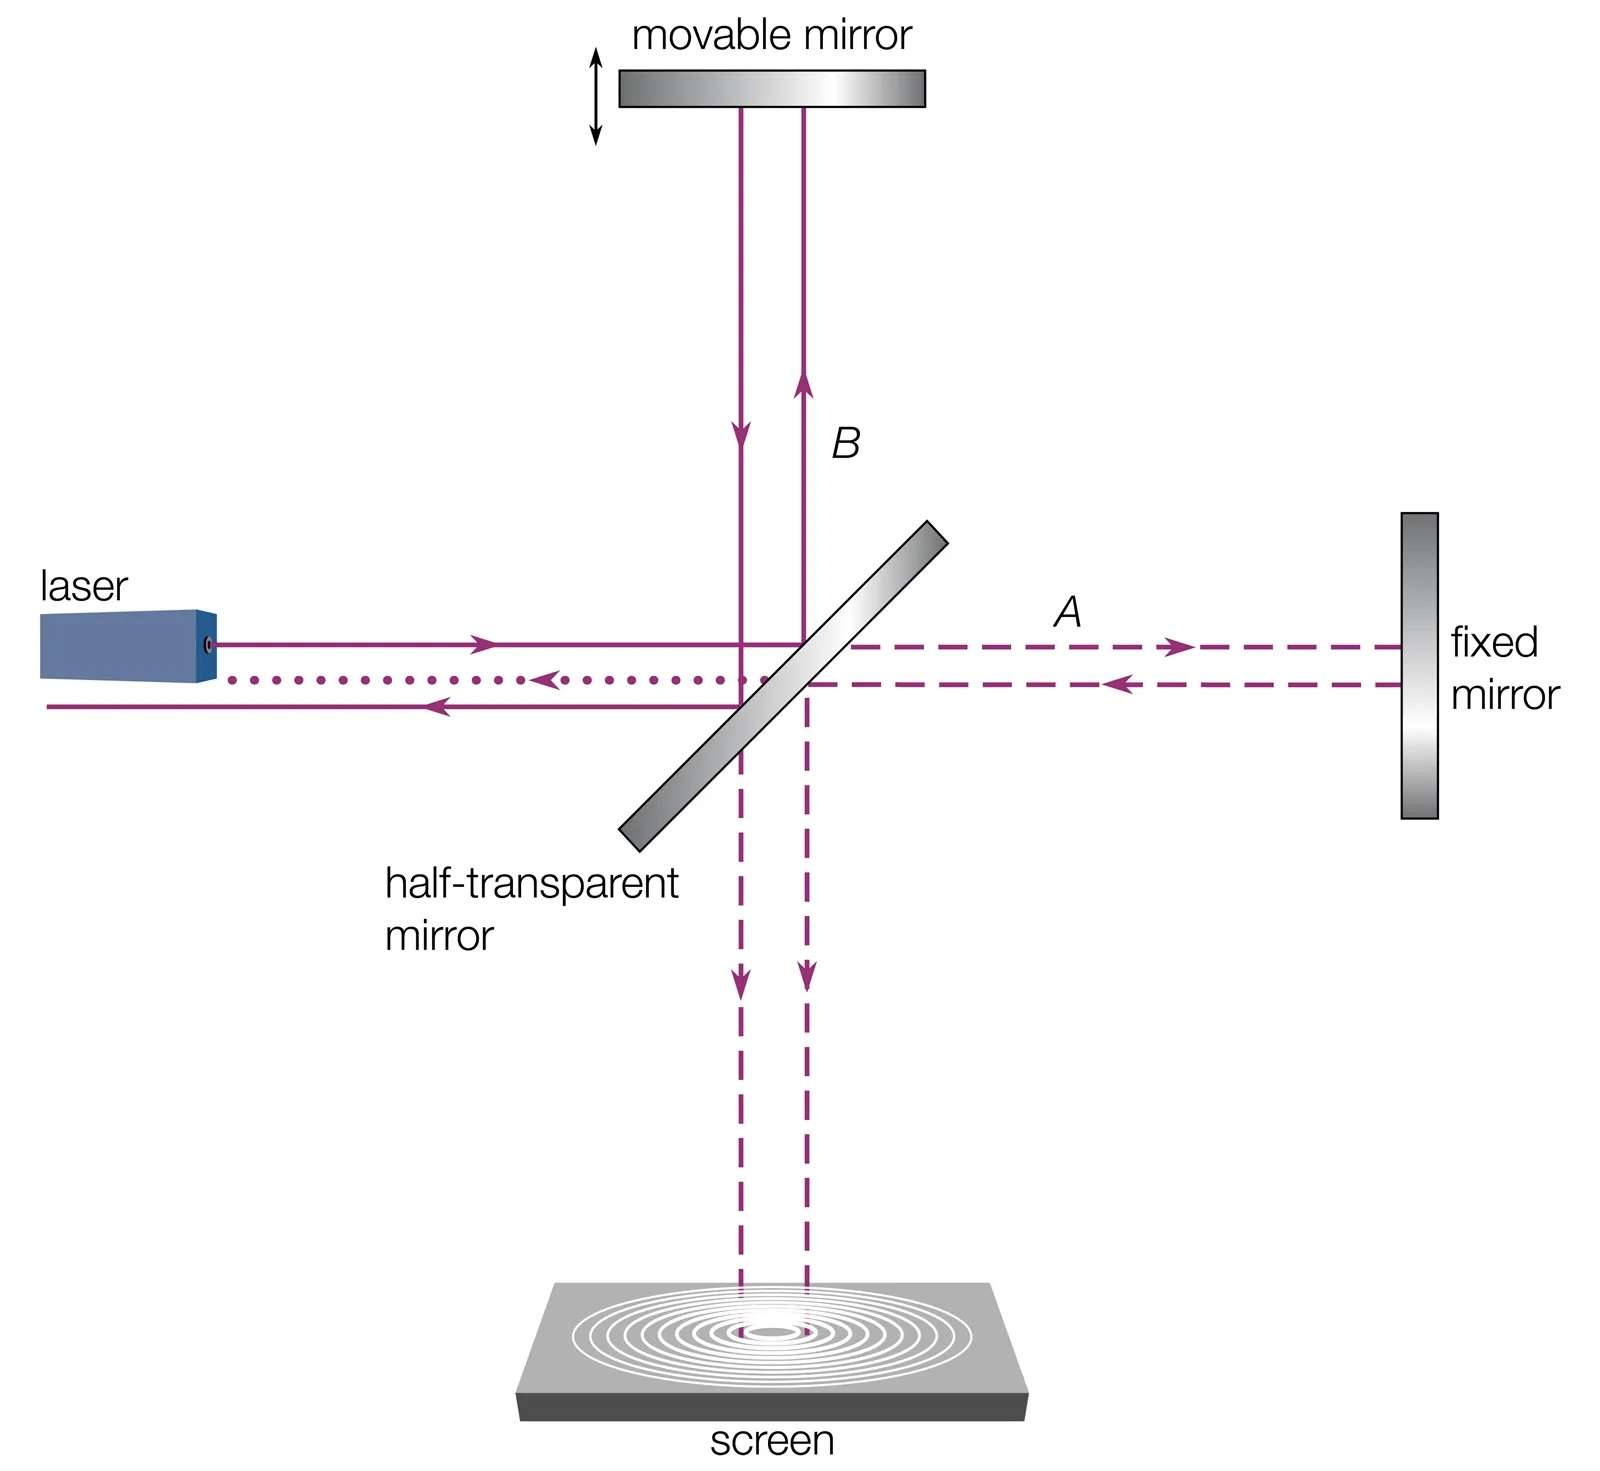
\includegraphics[width=6cm]{images/michelson_interferometer.png}
    \caption{Diagram of a michelson interferometer as used in LIGO.$^1$}
    \label{fig:michelson}
    \end{figure}
By using a michelson interfermoeter in the LIGO experiment the small changes in
distance that are required can be detected and measured. These distances can be on the
order of 10$^{-21}$m, caused by the passing of gravitational waves through the
interferometer arms. The first detection of a gravitational wave come on the 14th of
September 2015, just 100 years after the publicqtion of Einstiens paper.
The first detection was of a binary black hole merger, these mergers commonly
release a large amount of energy in the form of gravitational waves. This happens
because as the two black holes accelerate towards each other they warp the
space-time around them, and as the approach the point of coalescence the amplitude
of these waves massively increases, thus allowing them to be detected over the Background
noise. The run-down after merging is extremely quick and thus leaving a distinct peak
at the time of coalescence.


\section*{}




\section*{Method}




\section*{Results}



\section*{Analysis}




\newpage
\section*{Introduction and Background}

\section*{Aims}



\section*{Method}

\section*{Results}

\section*{Analysis}


\section*{Conclusion}

\section*{References}
\end{document}
